\documentclass[conference]{IEEEtran}
%\IEEEoverridecommandlockouts
% The preceding line is only needed to identify funding in the first footnote. If that is unneeded, please comment it out.
\usepackage{cite}
\usepackage{amsmath,amssymb,amsfonts}
\usepackage{algorithmic}
\usepackage{graphicx}
\usepackage{textcomp}
\usepackage{xcolor}
\def\BibTeX{{\rm B\kern-.05em{\sc i\kern-.025em b}\kern-.08em
    T\kern-.1667em\lower.7ex\hbox{E}\kern-.125emX}}

\usepackage[switch]{lineno}
\usepackage{stmaryrd}
\usepackage{float}
\usepackage{cite}
\usepackage{hyperref}
\usepackage{tabularx,booktabs,longtable}

\usepackage{listings}     
\usepackage{lstautogobble}  % Fix relative indenting
\usepackage{color}          % Code coloring
%\usepackage{zi4}            % Nice font

\definecolor{bluekeywords}{rgb}{0.13, 0.13, 1}
\definecolor{greencomments}{rgb}{0, 0.5, 0}
\definecolor{redstrings}{rgb}{0.9, 0, 0}
\definecolor{graynumbers}{rgb}{0.5, 0.5, 0.5}

\usepackage{listings}
\lstset{
	autogobble,
	columns=fullflexible,
	showspaces=false,
	showtabs=false,
	breaklines=true,
	showstringspaces=false,
	breakatwhitespace=true,
	escapeinside={(*@}{@*)},
	commentstyle=\color{greencomments},
	keywordstyle=\color{bluekeywords},
	stringstyle=\color{redstrings},
	numberstyle=\color{graynumbers},
	basicstyle=\ttfamily\footnotesize,
	frame=l,
	framesep=12pt,
	xleftmargin=12pt,
	tabsize=4,
	captionpos=b
}

\begin{document}
\linenumbers
\title{Empirical study of partial evaluation of matrix and string algorithms\\

\thanks{Identify applicable funding agency here. If none, delete this.}
}

\author{\IEEEauthorblockN{Ilya Balashov}
\IEEEauthorblockA{\textit{Saint Petersburg State University} \\
7/9 Universitetskaya nab., \\ St. Petersburg, 199034 Russia \\
i.balashov@2017.spbu.ru}
\and
\IEEEauthorblockN{Semyon Grigorev}
\IEEEauthorblockA{\textit{Saint Petersburg State University} \\
7/9 Universitetskaya nab., \\ St. Petersburg, 199034 Russia \\
s.v.grigoriev@spbu.ru
}
\and
\IEEEauthorblockN{Daniil Berezun}
\IEEEauthorblockA{\textit{Saint Petersburg State University} \\
7/9 Universitetskaya nab., \\ St. Petersburg, 199034 Russia \\
d.berezun@2009.spbu.ru}
}
\maketitle

\begin{abstract}
	
This paper describes the empirical study on the partial evaluation technique applied to execution time optimization of general matrix and string algorithms. We used AnyDSL framework for partial evaluation during the experiments. Execution time of non-optimized code is compared with the results of partially evaluated code and execution times of commonly used tools. An insides on existing work and our future plans are provided. Selection of algorithms, datasets and experiments structure were clarified. The results shows that partial evaluation with AnyDSL framework results in up to 1000 times execution time reduction on several cases for the selected matrix and string algorithms.
	
\end{abstract}

\begin{IEEEkeywords}
Partial evaluation, compilers, program optimization, specialization, automatic program transformation, linear algebra-based algoritms
\end{IEEEkeywords}

\section{Introduction}
Recent years have seen a significant increase in the sizes and complexity of programs in different areas of software engineering. Huge programs or libraries often contain some core code on which significant parts of the program depend, so this code needs to be highly optimized. However, creating a code with sufficiently low complexity for satisfying performance requirements is often an outstanding and time-consuming problem for an ordinary software engineer. A possible way of ensuring sufficient performance or such a code while keeping the development process comfortable for a programmer is the usage of automatic optimization tools and techniques, operating with program sources.

For instance, the so-called \textit{partial evaluation} (or specialization) \cite{jones1993partial} technique is being actively used over the last years as a way to optimize program execution time automatically, using data known statically. A special tool named \textit{partial evaluator} (or specializer) analyzes data (for example, function parameters) which was provided ahead of evaluation time, and applies several program optimization techniques to the code based on the structure of this data. 


Existing results in the area of applied usage of partial evaluation for automatic code optimization include image processing \cite{leissa2018anydsl}, bioinformatics \cite{muller2020anyseq} and ray tracing algorithms \cite{perard2019rodent}.


In this paper, we applied partial evaluation technique to a code of several algorithms usually utilized as core algorithms in areas connected with linear algebra and string processing. Experiments on partial evaluation of some matrix and string algorithms with AnyDSL \cite{leissa2018anydsl} framework and evaluating the suitability of the approach for application in industrial libraries and tools are provided. For each algorithm we described the datasets used and justified theoretical reasons why the algorithm could be successfully partially evaluated using AnyDSL tool. A compact overview of current research in the area and an inside on our future plans was also provided.

As a result, it is showed that partial evaluation with AnyDSL could successfully improve code performance in the general cases.


\section{Background}

\subsection{Partial evaluation}

Let's suppose:

\begin{itemize}
	\item $P$ is a program, which takes values $a_n\ [n=1..m]$ as an input
	\item $mix$ is a program which is defined as $mix\ [P, a_1] = P_a$
	\item $\llbracket P \rrbracket [a_1, a_2, .., a_m] = \llbracket P_a \rrbracket [a_2, .., a_m]$
\end{itemize}
Then the transformation of $P$ and $a_1$ to $P_a$ using $mix$ is called \textit{partial evaluation} \cite{jones1993partial}. Program $mix$ is called \textit{partial evaluator}. In other words, partial evaluation is a technique for evaluating parts of the program ahead of compilation with the usage of static input data.

A classic example of partial evaluation is the evaluation of power function. Code with linear complexity from Listing \ref{lst:power} could be partially evaluated using the knowledge of static power. So, assuming $n = 5$ code with constant complexity on Listing \ref{lst:power5} could be received.

\begin{lstlisting}[caption={Power function before evaluation},label={lst:power}]
fn power(x, n):
	if x == 1:
		x
	else:
		x * power(x, n - 1)
\end{lstlisting}

\begin{lstlisting}[caption={Power function partially evaluation using n = 5},label={lst:power5}]
fn power5(x):
	x*x*x*x*x
\end{lstlisting}


Despite partial evaluation is initially being used by Ershov \cite{ershov1982mixed}, Jones \cite{jones1993partial} and other scientist in their work for compiler generation via Futamura projections \cite{futamura1983partial}, it could also be used for program optimization. For instance, a partial evaluator can employ static data to unfold loops and conditional operators, propagate constants, etc \cite{jones1993partial}. 

% Difficulties of PE
However partial evaluation is a powerful method of program optimization, it is inherent in several difficulties. Firstly, a partial evaluator could inflate source code size heavily because of transformation such as loop unfolding and static data substitution. Therefore, evaluation results (code structure, bottlenecks, etc.) \textcolor{red}{formal} assessment becomes a non-trivial problem very often. To solve this issue in some degree, modern tools like AnyDSL \cite{leissa2018anydsl} tends to translate evaluated code into some intermediate representation which is often much easier to understand and analyze. Secondly, divergent program partial evaluation with the application of average-quality tool may lead to the evaluation process divergence \cite{jones1993partial}. So, the programmer has to be very careful while using this technique for optimization purposes. Finally, partial evaluation imposes serious requirements on the programmer qualification: a deep understanding of the evaluation process is highly required. To solve the issue modern tools are introducing simplified language constructions, such as a special partial evaluation wrapper \cite{leissa2018anydsl}, attribute-driven evaluation \cite{10.1007/978-3-319-74313-4_27} and many other various and creative methods.

\subsection{Matrix algorithms}

Algorithms on matrices (matrix-matrix, matrix-vector multiplication, tensor product, etc.) are very common in programs connected with linear algebra and linear algebra packages (BLAS).

For example, it is widely known that many graph algorithms could be explained in the language of matrices \cite{kepner2011graph,davis2019algorithm}. Linear algebra allows constructing algorithms like Breadth-First Search or Shortest Path Search with the exploitation of basic linear algebra operations: matrix multiplication, Kronecker product and some other algorithms. Therefore, if it was possible to speed up different matrix multiplication algorithms, it should be possible to speed up a large class of algorithms. 

One of the possible basic sets of linear algebra algorithms and operations for graph algorithm construction is named \textit{GraphBLAS} standard \cite{davis2019algorithm,moreira2018implementing}. For our experiments we chose \textit{matrix-matrix multiplication}, and \textit{Kronecker (tensor) product} algorithms \cite{cormen2009introduction}, which are considered as one of the core algorithms in GraphBLAS standard.

The results of matrix algorithms benchmarking are compared with the execution time of these algorithms implemented with SuiteSparse GraphBLAS library \cite{moreira2018implementing}, which is usually considered as the state-of-art implementation of GraphBLAS.

Before the experiments we predicted in theory that both of these algorithms could be successfully (without at least noticeable lose in performance) partially evaluated due to linear structure of their code and a relatively small number of conditional jumps in the proper implementation.


\subsection{Algorithms on strings}

Algorithms on strings are employed in different like regular expression handling or bioinformatics \cite{rajesh2010unusual}. One of the most common algorithms in this area are \textit{pattern matching} (substring search) and \textit{regular expression} (automaton) matching \cite{cormen2009introduction}, so we chose these algorithms for our experiments.

Also, a pattern matching algorithm is often utilized in so-called KMP-Test \cite{jones1993partial}. It shows how effectively the partial evaluator could optimize trivial substring search algorithm measured in a degree of efficiency approximation to Knuth-Morris-Pratt algorithm execution time. Therefore, partial evaluation of this algorithm could give us the essential data for the analysis.

We used adjacency matrices as regular expression automata representation since the matrix-based regular expression matching algorithm's code is in a more linear form, so we predict it should be evaluated better.

Existing results \cite{jones1993partial} shows that both of these algorithms could be successfully partially evaluated and AnyDSL tool is considered by us as a ``good enough'' tool to show this theoretically good result in practice.

\section{Algorithms implementation}

All algorithms were implemented using AnyDSL Impala domain-specific language \cite{leissa2018anydsl} for partial evaluation. AnyDSL framework was chosen due to its Impala DSL with comparatively simple Rust-like syntax and relatively available documentation. Algorithm code is represented as computation kernels, which is further linked with Google Benchmark-based \cite{gbenchmark} benchmarking code. Each algorithm was implemented in Impala twice: with partial evaluation language constructions and without them (therefore, with no partial evaluation).

Also, every algorithm was implemented with an alternative tool or framework that is usually used in practice for algorithm implementation in the corresponding area. In details, the following programs were used:
\begin{itemize}
	\item SuiteSparse GraphBLAS(link) --- for graph algorithms in the terms of linear algebra
	\item Grep and eGrep --- for algorithms on strings and regular expressions
\end{itemize}


All the code is placed on GitHub:
\begin{center}
\href{https://github.com/ibalashov24/spec\_experiments}{https://github.com/ibalashov24/spec\_experiments}
\end{center}

\section{Experimental design}

In this section, our experimental design for partial evaluation of selected algorithms using AnyDSL framework is described.

\subsection{Experimental setup}

Configuration of the experimental stand was:
\begin{itemize}
	\item Intel Core i5-7440HQ (4x3.8GHz) CPU
	\item 16Gb RAM
	\item Ubuntu 20.04
\end{itemize}

Tools' versions were fixed on the following commits from their official repositories:
\begin{itemize}
	\item Google Benchmark \cite{gbenchmark} --- commit dated 22 December 2020
	\item AnyDSL \cite{leissa2018anydsl} --- commit dated 8 December 2020
	\item SuiteSparse GraphBLAS \colorbox{red}{\cite{moreira2018implementing}} --- commit dated 14 July 2020
\end{itemize}

Default (e)Grep from Ubuntu 20.04 was employed.

We used Harwell-Boeing matrix collection \cite{duff1992users} (a subset of it is also known as SuiteSparse matrix collection \cite{davis2011university}) because it contains a reasonably diverse set of matrices. COO (COOrdinate list) sparse matrix format was used. In details, we got (both matrix-matrix product and Kronecker product) 4 sparse matrices taken from these sets: \textit{bcsstk16}, \textit{fs1831}, \textit{2blocks} and \textit{eye3}. First 2 of them could be considered as big and the last 2 are relatively small. \textit{bcsstk16} and \textit{2blocks} are of average structure without boundary cases, while  the elements of \textit{fs1831} and \textit{eye3} are concentrated near the main diagonal. Our benchmark used ``small'' matrices \textit{2blocks} and \textit{eye3} as static data during partial evaluation to prevent output code ramification and performance overhead creation.

For string algorithms, we used random strings and traffic dumps as sources and random strings or Latin words as patterns in order to show the results in a near-average case. Regular expressions (finite automata) were converted to COO sparse representation with our modification of Re2dfa tool \cite{re2dfa}. Our benchmark used ``short'' strings with the length smaller than 200 characters as static data to avoid generated code ramification and overhead creation.

AnyDSL partial evaluation tool was executed in JIT-mode \colorbox{red}{\cite{leissa2018anydsl}}, which allows to perform partial evaluation at the run time.



\subsection{Research questions}

To evaluate our approach, we design experiments to address the following research questions:

\begin{itemize}
	\item[\textbf{Q1:}] Does partial evaluated benefits string and matrix-based graph algorithms performance (execution time) comparing to their basic versions?
	\item[\textbf{Q2:}] In which degree partially evaluated algorithms code performance gets closer to their state-of-art implementations?
\end{itemize}

\subsection{Result metrics}
To evaluate the performance of partially evaluated code, we adopt the following widely used metrics for application performance:
\begin{itemize}
	\item \textbf{Execution time} is computed by the Google Benchmark tool and measured in nanoseconds. For each algorithm, the tool gives three numbers: time spent in real life, time spent on CPU, and iteration number. We took \textit{time spent in real life} to consider all hardware delays (for example, memory access delays).
	
	The smaller execution time is better.
	
	\item \textbf{Measure error} is computed by the Google Benchmark tool and measured in percents. 
	
	Numbers smaller than $0.01\%$ are considered a good result which guarantees a relatively small threat to validity.

\end{itemize}

\section{Results}
This section presents our experimental results by addressing the research questions.

\subsection{Does partial evaluation with AnyDSL benefits string and matrix-based graph algorithms performance comparing to their basic versions?}


\begin{table*}[!h]
\begin{tabular}{lccccc}

		Time, ns.   & bcsstk16 x 2blocks & bcsstk16 x eye3 & fs1831 x 2blocks & fs1831 x eye3 \\
		\multicolumn{5}{c}{Matrix-Matrix product}                                             \\
		No spec     & 3569461            & 152191          & 48082            & 7526          \\
		Spec        & 172553             & 94126           & 20487            & 8025          \\
		SuiteSparse & 5302               & 1825            & 1825             & 2056          \\
		\multicolumn{5}{c}{Kronecker product}                                                 \\
		No spec     & 186                & 126550          & 22509            & 966           \\
		Spec        & 34.5               & 157196          & 2016             & 893           \\
		SuiteSparse & 198                & 199             & 197              & 199          
\end{tabular}
\centering
\caption{Execution time comparison of matrix algorithms non-specialized code (No spec),\\ specialized code in AnyDSL Impala (Spec), code implemented with model tool (SuiteSparse)}
\label{table_graph}
\end{table*}



\begin{table*}[]
	\begin{tabular}{llll}
		Time, ns       & Big source 1 & Big source 2 & Small pattern \\
		No spec        & 33129202     & 28983335     & 2413          \\
		Spec           & 11757516     & 11686216     & 922           \\
		Grep (approx.) & 24000000     & 50000000     & 1000                   
	\end{tabular}
	\centering
	\caption{Execution time comparison of pattern matching non-specialized code (No spec),\\ specialized code in AnyDSL Impala (Spec) \\ and approximate time (the tool output is in integer ms) for code implemented with model tool (Grep)}
	\label{table_string}
\end{table*}

\begin{table*}[]
	\begin{tabular}{llll}
		Time, ns        & Email (weak) & Email        & Credit card \\
		No Spec         & 1273112850   & 1951322141   & 1824        \\
		Spec            & 1623176      & 2223887      & 23.2        \\
		eGrep (approx.) & 118945000000 & 174746000000 & 69000000          
	\end{tabular}
	\centering
	\caption{Execution time comparison of regular expression (automata) search non-specialized code (No spec),\\ specialized code in AnyDSL Impala (Spec) \\ and approximate time (the tool output is in integer ms) for code implemented with model tool (eGrep)}
	\label{table_regex}
\end{table*}

As seen from Table \ref{table_graph} and Figure \ref{fig:multpe}, partial evaluation gives significant, more than several times, speed up on test cases involving \textit{2blocks} as right \textcolor{red}{multiplicator}. It may be explained with relatively distributed structure of \textit{2blocks} matrix non-zero elements, that allows partial evaluator to effectively perform optimizations like loop unfolding and constant propagation.\\
In contrast, non-zero elements of \textit{eye3} matrix are concentrated near the main diagonal of the matrix which leads to relatively small execution time benefit (or absent) of partial evaluation --- loop unfolding does not discard any empty iterations.

\begin{figure}[H]
	\centering
	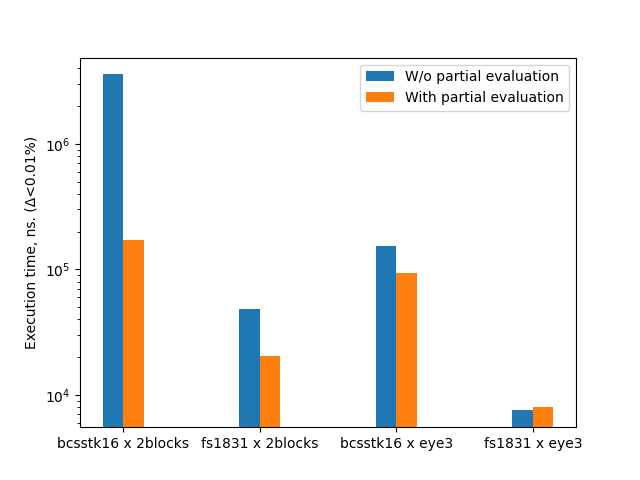
\includegraphics[scale=0.6]{matrix-mult}
	\caption{Comparison of matrix-matrix multiplication algorithm execution times before and after partial evaluation}
	\label{fig:multpe}
\end{figure}

For string algorithms, we may observe a much more noticeable execution time increase after a partial evaluation than in graph algorithms. As could be seen from Table \ref{table_string} and Table \ref{table_regex}, the speed up lays between 10 and 100 times depending on the test. The reason for such a significant increase is that the most of iterations in classic substring search and pattern matching algorithms \cite{cormen2009introduction} with matrix input is not empty, like in previously discussed algorithms on sparse matrices graphs. Also, in substring search algorithm evaluation is simplified by the fact that the data is being iterated successively.\\
Moreover, there is an absent of non-logical operations with both source and pattern data as operands in these algorithms, so the partial evaluator can apply constant propagation optimization heavily due to trivial data separation.

The results show that in general partial evaluation with AnyDSL benefits string and matrix-based graph algorithms execution time comparing to their basic versions.

%\begin{figure}[H]
%	\centering
%	\includegraphics[scale=0.5]{../../LinearAlgebraImpala/MatrixMultiplication/Charts/jit_drawer/prod_suitesp}
%	\caption{Execution time of matrix multiplication algorithm comparison between SuiteSparse and partially evaluated code using AnyDSL}
%\end{figure}

\begin{figure}
	\centering
\end{figure}

\subsection{In which degree partially evaluated algorithms code performance gets closer to their state-of-art implementations?}

Tables \ref{table_graph}, \ref{table_string} and \ref{table_regex} show the time (in nanoseconds) of execution of matrix-based graph and string algorithms respectively. 

For the string algorithms, we can see that partially evaluated code outperforms Grep (for pattern matching) and eGrep (for regular expressions matching) in several times (2 to 10000) on each of the datasets. However AnyDSL beat (e)Grep in both pattern and regular expression matching problems, we could see that the latter gave by several orders of magnitude stronger results. According to our analysis, it could be the result of using COO representation for regular expression's transition graph in the experiment: linear structure of a COOrdinate list structure allows the partial evaluator to use more aggressive optimizations such as \textcolor{blue}{vectorization} or easier loop unfolding.

For graph algorithms in a matrix form (matrix multiplication and Kronecker product), we may \textcolor{red}{observe} that partially evaluated algorithms' code underperforms code of the same algorithms implemented with SuiteSparse GraphBLAS \textcolor{red}{in} 10 times in average. It could be considered a good result, since non-partially evaluated code loses 100 times in half of cases.

To sum up, for the selected string algorithms partially evaluated code outperforms their industrial implementations by execution time in a high degree; for the selected graph algorithms in matrix form partially evaluated code lags behind their state-of-art implementation by a factor of 10 (which is a good result).

\subsection{Conclusion}
As a result, partial evaluation of several matrix and string algorithms usually used as core algorithms in different programs or libraries shows relatively good results. So, we could conclude that partial evaluation (at least, with AnyDSL framework) could be successfully applied as a helper technique for a programmer, who intends to automatically optimize algorithmic code in high-loaded systems.


\section{Threats to validity}

\subsection{Subject selection bias}
In our research, we use only AnyDSL framework for the experiments. Other partial evaluation tools may give slightly different results due to more or less aggressive optimizations or different evaluation techniques.

\subsection{Used datasets}
Despite trying to run experimental code on both versatile and special datasets, we admit that partially evaluated code could give slightly different measures on some other special degenerate matrix sets.

\section{Related work}

Partial evaluation of linear algebra (especially matrix algorithms) was studied before in several papers.

Firstly, it is measured \cite{tyurin2020optimizing} that partial evaluation of matrix convolution and pattern matching algorithms using AnyDSL framework and CUDA reduces execution times up to 8 times on most datasets.

Secondly, partial evaluation was applied for Viterbi algorithm optimization \cite{viterbiseim}. It was discovered that the evaluated version of the code outperforms the non-evaluated one by 1.5 times in some cases.

Moreover, AnyDSL team performed research \cite{perard2019rodent} on the application of partial evaluation for ray tracing purposes in their library named Rodent. It was measured that partial evaluation makes an improvement in execution time of around $25\%$ on selected datasets.

Also, several other partial evaluators could be used instead of AnyDSL for matrix and string algorithms code optimization. For instance, it could be LLVM.mix, which was successfully applied for database query optimization \cite{sharygin2017runtime}, or C-mix \cite{jones1993partial}.

\section{Future work}

In short term, we are planning to set up the experiments on more complex algorithms: shortest path algorithm and breadth-first search.

Also, there is an interesting task to translate our experiments' code into a new AnyDSL frontend language named Artic \cite{articgit}. It allows parametric polymorphism, so it should be possible to implement semirings support, which is essential for algorithms on graphs in matrix representation.


\bibliographystyle{ieeetran}
\bibliography{syrcose}

\end{document}
